\documentclass[12pt, english]{scrartcl} %Koma-Klasse "Artikel" mit 12pt Schrift
\usepackage[left=20mm, right=20mm, top= 25mm, bottom=25mm]{geometry}  % Seitenrändern
\usepackage{graphicx} %zum Einfügen von Bildern
\usepackage[english]{babel} %englische Silbentrennung
\usepackage{multicol}
\usepackage{graphicx}
\usepackage{caption}
\graphicspath{graphics/}
\usepackage{siunitx}

\sisetup{separate-uncertainty}
\usepackage{braket}

\title{F18/38 Atmospheric Spectroscopy}
\author{Carsten L{\"u}th \and Michael Dorkenwald}
\date{\today}

\begin{document}
\maketitle

\begin{multicols}{2}


\section{Abstract}
In this experiment the trace gases Nitrogendioxid ($NO_2$) and Ozone ($O_3$) are examined with DOASIS. These gases play an important role for life on earth. Therefore it is important to have a method to determine the concentration in the air. The DOASIS (DOAS Intelligent System) was developed at the Institut for Environmental physics at University Heidelberg
\section{Introduction}
The atmosphere is the gas cover surrounding an astronomic object due to its gravitation. The experiment on which this report is based analyses the atmosphere of the earth and how we humans interact with it by the usage of fossil fuels.\\
The earth's atmosphere is divided into troposphere, stratosphere, mesosphere, thermosphere and exosphere. The UV-radiation of the sun is almost purely absorbed (roughly $95-99\%$) in the stratosphere by the gas ozone ($O_3$). 
Due to the emission of climate gases or radicals for catalytic ozone destruction such as $NO$ humans impacted the concentration of $O_3$ in stratosphere and troposphere.\\  
This lead to the creation of the Ozone-hole over antarctica (and the arctica) as well as health issues in urban or strongly industrialized areas due to photochemical smog.\\
The overarching goal of the experiments was it to analyse the $O_3$ and $NO_2$ concentrations over the course of the day and their spatial arrangement.\\
All measurements in this experiment were done with the \textbf{D}ifferential \textbf{O}ptical \textbf{A}bsorption \textbf{S}pectroscopy method. 
First we conducted a mini experiment with a $NO_2$ gas-cell to learn the basis functions of our spectrometer and the methods used in combination to measure the \textbf{S}lant \textbf{C}olumn \textbf{D}ensity with an active source of light.\\
Second we did a Zenith sky measurement to determine the \textbf{V}ertical \textbf{C}olumn \textbf{D}ensity of $O_3$ and $NO_2$ over the course of a day. 
In the last measurement we used the principle of Multi-Axis-DOAS by measuring the SCD for different elevation angles the incoming light to determine the density of $O_3$, $O_4$ and $NO_2$ in the troposphere.\\
\section{Background}
In the following the most important principles to understand our measurements and conclusions are briefly introduced and a bit of reasoning for their importance.
\subsection{Ozone and Nitrogendioxid}
The $O_3$ concentration in the air is the result of an equilibrium for creation and destruction of $0_3$ molecules. Most of the $O_3$ from a VCD is located in the stratosphere because the $O_2$ photolysis is part of the reaction to create $O_3$. The probability a $O_2$ photolysis scales with the density of $O_2$ and requires a photon with a wavelength smaller then $242nm$ which mostly get absorbed by the photolysis happening in the stratosphere.\\
To predict the VCD of $O_3$ two theoretical models are used together. The Chapman Cycle describes the reactions between $O_2$, $O_3$ and photons. While the Catalytic ozone destruction describes how radicals of the groups $HO_X$ ($H, OH, HO_2$), $NO_X$ ($NO_2,NO$), $ClO_X$ ($Cl, ClO$) and $BrO_X$ ($Br,BrO$) greatly accelerate the ozone destruction. These radicals can cycle through thousands of iterations of the accelerated destruction cycle, while only being removed by chemical reactions or sedimentation.\\
$NO_2$ being one of those radicals is mainly a secondary pollutant, meaning that it is not a direct emission of burning fossil fuels. Instead it is mainly produced by a reaction between $NO$ and $O_3$. The most important mechanism for the formation of $NO$ is the Zel'Dovic cycle describing the \textit{thermal} formation of $NO$, the reaction between very high energetic $N_2$ and $O_2$.\\
The oxidation to $NO_2$ is explained by equations \ref{o3recomb} - \ref{photolysis} which result in the \textbf{photostationary state} between $O_3$ and $NO_X$.
\begin{equation}\label{o3recomb}
O + O_2 + M \rightarrow O_3 + M 
\end{equation}
\begin{equation}\label{steady}
O_3 + NO \Longleftrightarrow NO_2 +O_2
\end{equation}
\begin{equation}\label{photolysis}
NO_2 + h\nu(\lambda < 410 nm) \rightarrow NO + O
\end{equation}
The molecule or atom $M$ is only needed for the conservation of momentum.
The steady state resulting from the photostationary state can be described by the \textbf{Leighton ratio} (eq. \ref{Leighton}).
\begin{equation}\label{Leighton}
\frac{[NO]}{[NO_2]} = \frac{j_{NO_2}}{k_{O_3+NO} \cdot [O_3] }
\end{equation}
The photolysis rate, depending on sun angle and intensity, is described by $j_{NO_2}$ and  $k_{O_3+NO}$ is the reaction constant in equation \ref{steady}.\\
\paragraph{Diurnal Cycle}
During a day the $NO_2$ and $NO$ concentrations change cyclically due to the building of $NO_3$ and $NO_5$. In the \textit{morning} the mixing ratio of $NO_2$ in the stratosphere increases due to the dissociation of $NO_5$ excited by photons. During the \textit{day} $NO$, $NO_2$ and $O_3$ are in a photostationary balance and in the \textit{evening} the photolysis (eq. \ref{photolysis}) decreases and $NO$ is no longer created, leading to an increase of $NO_2$. At \textit{night} $NO_2$ forms $NO_5$ again.
\paragraph{Photochemical smog}
Photochemical smog occurs when high levels of volaticle organic compounds (VOCs) and $NO_X$ are emitted into thermal inversion layer so that are trapped closely to the ground. This leads to very high ozone levels in the troposphere because in the presence of VOCs there is another reaction path for the conversion of $NO$ to $NO_2$. The reaction between VOCs and $NO_X$ means that the Leighton ratio is no longer valid with the photostationary balance and destruction of $O_3$. 

 \subsection{The DOAS Measurement System}

\newpage
\section{Meassurements}
\subsection{Nitrogendioxid gas-cell}
In this part of the experiment we measured the absorption of a $NO_2$ gas-cell in the spectrum of an Hg-lamp. Due to the nature of this measurement we could simplify the problem by using the fact that we have access to $I_0$ by taking a spectrum without the gas cell in the light path and then take a measurement with the gas-cell in the light path to measure $I$. After dark current and offset were corrected for both measurements we used the simplified lambert-beer law to get to equation.
\begin{equation}
\tau = \log(\frac{I_0(\lambda)}{I_0(\lambda)})= \sigma_{NO_2} \cdot \rho \cdot L
\end{equation}
The reference convolution for $NO_2$ was then used to compute the SCD$= \rho \cdot L$. This was then used to compute the density $\rho = (2.81 \pm 0.07 ) \cdot 10^{-7} \frac{\text{mol}}{\text{cm}^3}$ and the mixture ratio $(6.29 \pm 0.39) \cdot 10^3 \text{ppm}$.
\subsection{Sunlight of a recorded daycycle}

\subsection{Sunlight different evaluations angles}

\section{Results}
\subsection{Nitrogendioxid gas-cell}
After dark current and offset were corrected for both measurements we used the simplified lambert-beer law to get to equation.
\begin{equation}
\tau = \log(\frac{I_0(\lambda)}{I_0(\lambda)})= \sigma_{NO_2} \cdot \rho \cdot L
\end{equation}
The reference convolution for $NO_2$ was then used to compute the SCD$= \rho \cdot L$. This was then used to compute the density $\rho = (2.81 \pm 0.07 ) \cdot 10^{-7} \frac{\text{mol}}{\text{cm}^3}$ and the mixture ratio $(6.29 \pm 0.39) \cdot 10^3 \text{ppm}$.


\subsection{Sunlight of a recorded daycycle}
The DOAS least squares fit computes the SCD values for the different daytimes and traces gases, namely ozone and nitrogendioxid. Those values were then plotted and can be seen in figures ...
\begin{figure}
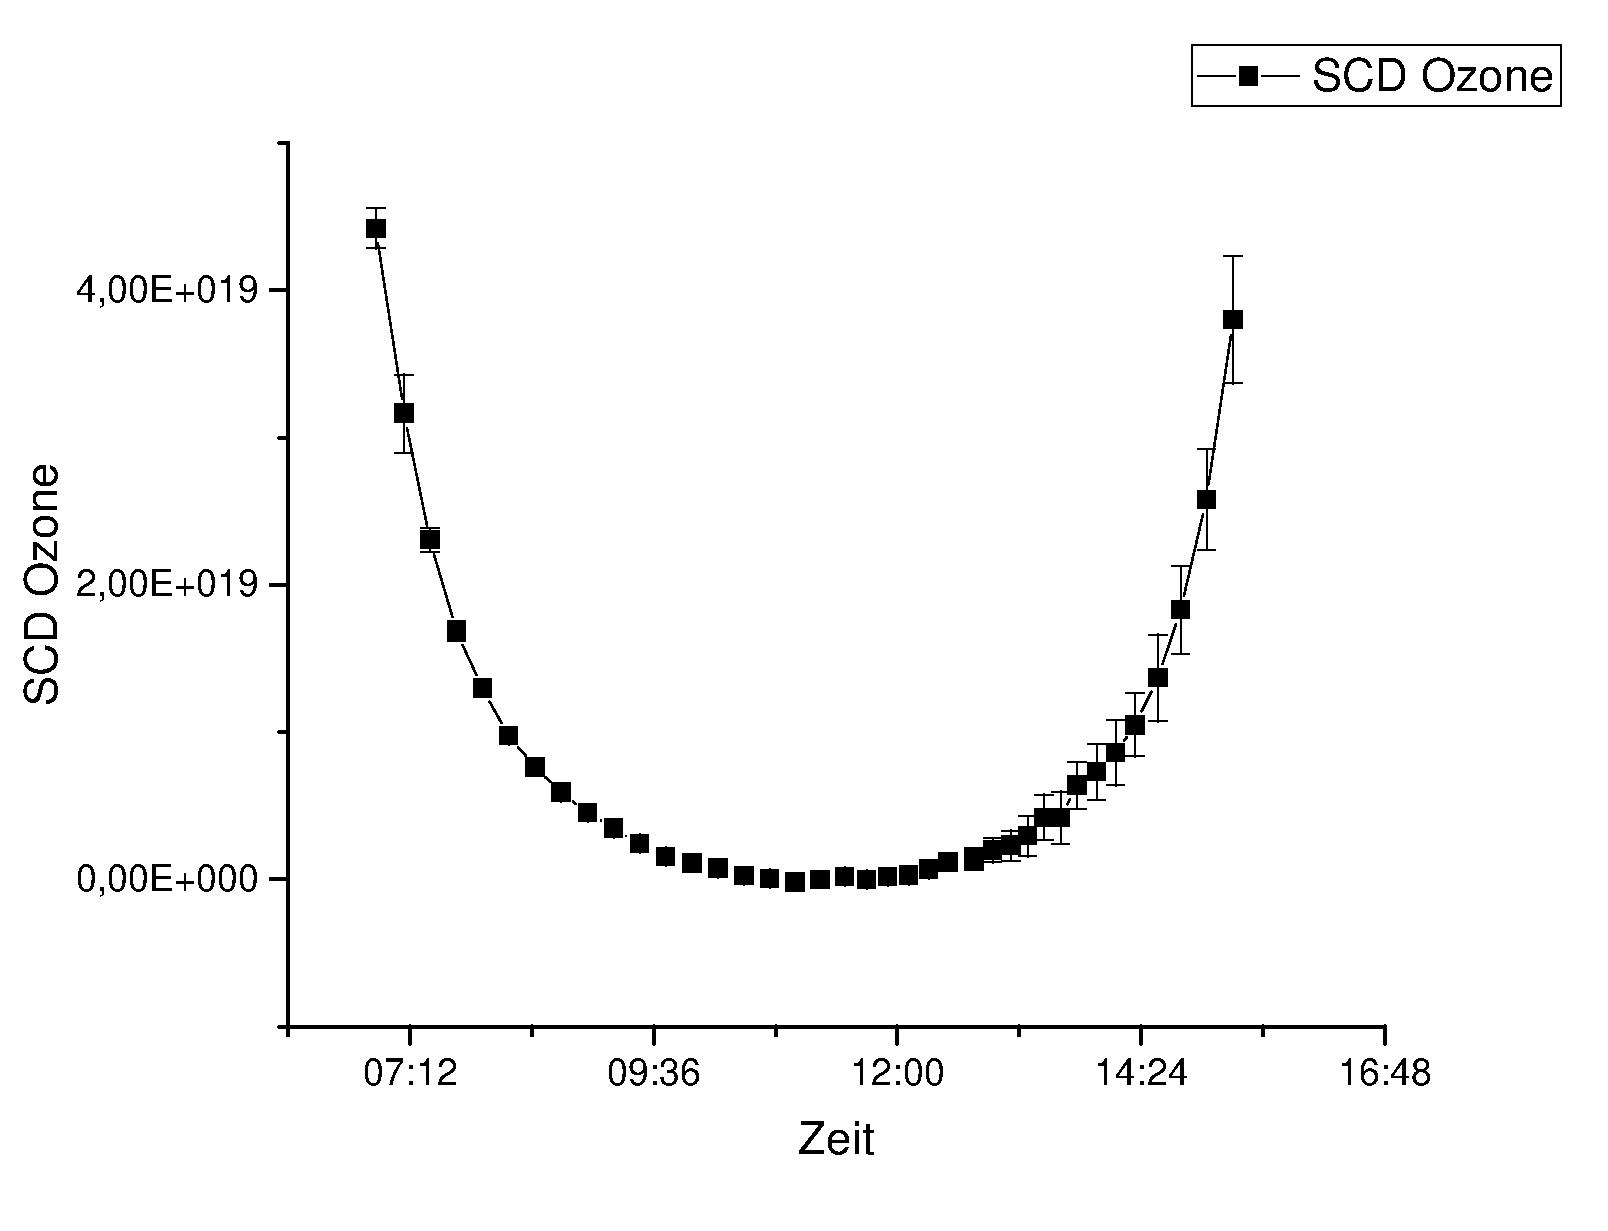
\includegraphics[width= 0.9\textwidth]{graphics/o3scd.pdf}
\end{figure}

\subsection{Sunlight different evaluations angles}


\section{Discussion}
\end{multicols}

\end{document}